\documentclass[]{book}
\usepackage{lmodern}
\usepackage{amssymb,amsmath}
\usepackage{ifxetex,ifluatex}
\usepackage{fixltx2e} % provides \textsubscript
\ifnum 0\ifxetex 1\fi\ifluatex 1\fi=0 % if pdftex
  \usepackage[T1]{fontenc}
  \usepackage[utf8]{inputenc}
\else % if luatex or xelatex
  \ifxetex
    \usepackage{mathspec}
  \else
    \usepackage{fontspec}
  \fi
  \defaultfontfeatures{Ligatures=TeX,Scale=MatchLowercase}
\fi
% use upquote if available, for straight quotes in verbatim environments
\IfFileExists{upquote.sty}{\usepackage{upquote}}{}
% use microtype if available
\IfFileExists{microtype.sty}{%
\usepackage{microtype}
\UseMicrotypeSet[protrusion]{basicmath} % disable protrusion for tt fonts
}{}
\usepackage{hyperref}
\hypersetup{unicode=true,
            pdftitle={Basic Read Alignment},
            pdfauthor={Dan MacLean},
            pdfborder={0 0 0},
            breaklinks=true}
\urlstyle{same}  % don't use monospace font for urls
\usepackage{natbib}
\bibliographystyle{apalike}
\usepackage{longtable,booktabs}
\usepackage{graphicx,grffile}
\makeatletter
\def\maxwidth{\ifdim\Gin@nat@width>\linewidth\linewidth\else\Gin@nat@width\fi}
\def\maxheight{\ifdim\Gin@nat@height>\textheight\textheight\else\Gin@nat@height\fi}
\makeatother
% Scale images if necessary, so that they will not overflow the page
% margins by default, and it is still possible to overwrite the defaults
% using explicit options in \includegraphics[width, height, ...]{}
\setkeys{Gin}{width=\maxwidth,height=\maxheight,keepaspectratio}
\IfFileExists{parskip.sty}{%
\usepackage{parskip}
}{% else
\setlength{\parindent}{0pt}
\setlength{\parskip}{6pt plus 2pt minus 1pt}
}
\setlength{\emergencystretch}{3em}  % prevent overfull lines
\providecommand{\tightlist}{%
  \setlength{\itemsep}{0pt}\setlength{\parskip}{0pt}}
\setcounter{secnumdepth}{5}
% Redefines (sub)paragraphs to behave more like sections
\ifx\paragraph\undefined\else
\let\oldparagraph\paragraph
\renewcommand{\paragraph}[1]{\oldparagraph{#1}\mbox{}}
\fi
\ifx\subparagraph\undefined\else
\let\oldsubparagraph\subparagraph
\renewcommand{\subparagraph}[1]{\oldsubparagraph{#1}\mbox{}}
\fi

%%% Use protect on footnotes to avoid problems with footnotes in titles
\let\rmarkdownfootnote\footnote%
\def\footnote{\protect\rmarkdownfootnote}

%%% Change title format to be more compact
\usepackage{titling}

% Create subtitle command for use in maketitle
\providecommand{\subtitle}[1]{
  \posttitle{
    \begin{center}\large#1\end{center}
    }
}

\setlength{\droptitle}{-2em}

  \title{Basic Read Alignment}
    \pretitle{\vspace{\droptitle}\centering\huge}
  \posttitle{\par}
    \author{Dan MacLean}
    \preauthor{\centering\large\emph}
  \postauthor{\par}
      \predate{\centering\large\emph}
  \postdate{\par}
    \date{2020-01-14}

\usepackage{booktabs}
\usepackage{amsthm}
\makeatletter
\def\thm@space@setup{%
  \thm@preskip=8pt plus 2pt minus 4pt
  \thm@postskip=\thm@preskip
}
\makeatother

\begin{document}
\maketitle

{
\setcounter{tocdepth}{1}
\tableofcontents
}
\hypertarget{about-this-course}{%
\chapter{About this course}\label{about-this-course}}

In this short course we'll look at a method for running an alignment of sequence reads against a reference genome. The course is very brief and will show you how to use a program called \texttt{minimap2} and \texttt{samtools} to create a binary alignment file that you can use in further work.

I acknowledge that there are lots of other programs and methods - this course is \emph{not} meant to be comprehensive, it is meant to get you being productive. Seek out further advice if you need to run other programs. Do be encouraged though, 99 \% of what you learn here will be applicable to other tools for the same job (they all run in a \emph{very} similar manner) so this is a good place to start.

The course has two main parts - first we'll learn to do this `locally', that is to say on the computer that you are actually physically sitting at and have direct control over. Once we've done that and know how to run the actual programs then we shall switch to running the programs `remotely' on a HPC environment using a submission system that you have to log in to.

\hypertarget{prerequisites}{%
\section{Prerequisites}\label{prerequisites}}

This course assumes that you are familiar with the basics of running stuff from a command-line. You'll need to have some experience not lots. If you've done the TSL command-line course you'll know plenty

For the first `local' part of this you'll need some software on your machines. Most bioinformatics software has to run on Unix style computers, which for most of us means Macs. The installation instructions below only apply to Macs.

For the second part you'll need an HPC account. See the Bioinformatics Team to get one of these.

\hypertarget{local-software-installation}{%
\subsection{Local Software Installation}\label{local-software-installation}}

We need to install \texttt{minimap2} and \texttt{samtools}. Installing bioinformatics software is often \emph{not} straightforward so we'll take a path of least resistance and install some tools that manage software for us. This is a roundabout way of doing things, but it greatly simplifies the hard parts and means that we can isolate our installations from the rest of our computer and not mess up anything already installed.

\begin{enumerate}
\def\labelenumi{\arabic{enumi}.}
\tightlist
\item
  \textbf{Get \texttt{conda}}
  \texttt{conda} is an environment and package manager for software projects (initially Python - hence the name). Its purpose is to create a sandbox area on your computer where you can safely install software without it interfering or overwriting any of the existing software already on there. This safe space is called a conda `environment'. To install \texttt{conda}:

  \begin{enumerate}
  \def\labelenumii{\arabic{enumii}.}
  \tightlist
  \item
    Click this link \url{https://repo.anaconda.com/miniconda/Miniconda3-latest-MacOSX-x86_64.pkg} and wait for the package to download. When it has double-click it and go through the installation process.
  \end{enumerate}
\item
  \textbf{Get \texttt{bioconda}}
  \texttt{bioconda} is plugin that makes \texttt{conda} aware of the bioinformatics software we will need. To make \texttt{conda} aware of \texttt{bioconda}

  \begin{enumerate}
  \def\labelenumii{\arabic{enumii}.}
  \tightlist
  \item
    Open \texttt{Terminal} and type the following:
  \end{enumerate}
\end{enumerate}

\begin{verbatim}
      conda config --add channels defaults
      conda config --add channels bioconda
      conda config --add channels conda-forge
\end{verbatim}

\begin{enumerate}
\def\labelenumi{\arabic{enumi}.}
\setcounter{enumi}{2}
\tightlist
\item
  \textbf{Create a new environment}
  We can now create our new safe space environment. Type in the following.
\end{enumerate}

\begin{verbatim}
      conda create --name alignment_env
\end{verbatim}

This step can take a moment or two and nothing seems to happen for a while - be patient. Accept the defaults (answer \texttt{y} when questioned).

\begin{enumerate}
\def\labelenumi{\arabic{enumi}.}
\setcounter{enumi}{3}
\tightlist
\item
  \textbf{Activate the environment}
  Everytime we want to use the new environment, including to install something into it, we have to activate it. That means each time we leave or start a new Terminal we need to type this into it
\end{enumerate}

\begin{verbatim}
  conda activate alignment_env
\end{verbatim}

You should see the name at the \texttt{\$} prompt change, telling you that this Terminal is in the \texttt{alignment\_env} environment. If you ever can't find programs that you're sure you installed, it means that you probably didn't activate the right environment.

\begin{enumerate}
\def\labelenumi{\arabic{enumi}.}
\setcounter{enumi}{4}
\tightlist
\item
  \textbf{Install the alignment software \texttt{minimap2} and \texttt{samtools}}
  All the steps up to now have been so we can do this one! Install each of the pieces of software in turn by using \texttt{conda} with:
\end{enumerate}

\begin{verbatim}
      conda install minimap2
      conda install samtools
\end{verbatim}

These steps can also take a while. Again accept the defaults (answer \texttt{y}).

Now you are done! Everything is installed ready for you to work with. Next we need to get the sample data

\hypertarget{sample-reference-genome-and-reads}{%
\subsection{Sample reference genome and reads}\label{sample-reference-genome-and-reads}}

You'll need this zip file of data: \href{https://github.com/TeamMacLean/basic_alignment/raw/master/sample_data/sample_data.zip}{sample\_data.zip} which contains a reference genome and some file and a set of paired end reads . Download it, extract the files and put them into a folder on your machine. I suggest something like \texttt{Desktop/align\_tut}. This will be the directory we'll work from in the rest of the course.

That's all you need to do the lesson. If you have any problems getting this going, then ask someone in the Bioinformatics Team and we'll help.

\hypertarget{intro}{%
\chapter{The Alignment Pipeline}\label{intro}}

In this chapter we'll look at an overview standard paired-end read run of \texttt{minimap2}, what it outputs and how to manipulate the output with \texttt{samtools}.

The overall pipeline is very straightforward\ldots{}

\begin{enumerate}
\def\labelenumi{\arabic{enumi}.}
\tightlist
\item
  Align all reads to a reference
\item
  Filter badly scoring reads
\item
  Sort and compress output
\end{enumerate}

\hypertarget{align-all-reads-to-a-reference}{%
\section{Align all reads to a reference}\label{align-all-reads-to-a-reference}}

This is the main step, and with \texttt{minimap2} it can be accomplished with a single command-line. In this step each read is aligned against the reference, and its best aligning position found. That position, along with a metric of the quality of the single alignment is reported in a \texttt{SAM} format file.

\hypertarget{filter-out-badly-scoring-reads}{%
\section{Filter out badly scoring reads}\label{filter-out-badly-scoring-reads}}

This is the quality control step. We remove reads that don't have a good alignment score because in most contexts it means the read is a bad read with bad sequence in it. Of course in some contexts it isn't - it depends what you're aligning to what, but for the RNAseq situation or SNP calling situation where we expect the reads to be very like the reference this is appropriate. This step is done with \texttt{samtools}

\hypertarget{sort-and-compress-output}{%
\section{Sort and compress output}\label{sort-and-compress-output}}

Once filtering is done and we have the set of reads we wish to retain we can take our output file and convert it to a sorted binary format that uses less disk space and is optimised for searching in downstream analysis. This step is a kind of housekeeping step that makes everything later easier. We do it with \texttt{samtools}

\hypertarget{further-reading}{%
\section{Further Reading}\label{further-reading}}

\hypertarget{fastq-quality-scores}{%
\subsection{FastQ quality scores}\label{fastq-quality-scores}}

Typically the reads we use will be in the FastQ format, this is a two line format that encodes not only the sequence read, but the `believability' of each base. You can see more \href{https://en.wikipedia.org/wiki/FASTQ_format}{here}

\hypertarget{why-minimap2-and-not-bwabowtieother}{%
\subsection{Why minimap2 and not bwa\textbar{}bowtie\textbar{}other}\label{why-minimap2-and-not-bwabowtieother}}

You may have heard of other aligners and that people in your group are using them. \texttt{minimap2} is currently the quickest and most accurate of all the aligners and has general ability with all modern sequence types. Those using others (in particular bwa and bowtie) are pretty out of date. bwa \emph{was} a favourite for a long time, but has been superceded. The same author created both bwa and minimap2 and minimap2 was written to address issues with bwa.

\hypertarget{running-minimap2}{%
\chapter{\texorpdfstring{Running \texttt{minimap2}}{Running minimap2}}\label{running-minimap2}}

Running \texttt{minimap2} takes only one step. Assuming we've already \texttt{cd}'d into the directory with the reads and reference we can use this command

\begin{verbatim}
  minimap2 -ax sr ecoli_genome.fa ecoli_left_R1.fq ecoli_right_R2.fq > aln.sam
\end{verbatim}

Try running that and see what happens\ldots{} You should get an output file in the working directory called \texttt{aln.sam}. On my machine this takes just a few seconds to run.

Let's look at the command in detail.

\hypertarget{the-minimap2-command-and-options}{%
\section{\texorpdfstring{The \texttt{minimap2} command and options}{The minimap2 command and options}}\label{the-minimap2-command-and-options}}

First we get this

\begin{verbatim}
  minimap2
\end{verbatim}

which is the name of the actual program we intend to run, so it isn't surprising that it comes first. The rest of the command are options (sometimes called arguments) telling the program how to behave and what it needs to know. Next up is this

\begin{verbatim}
           -ax sr
\end{verbatim}

which gives option \texttt{a} meaning print out SAM format data. And option \texttt{x} meaningwe wish to use a preset parameter set. The preset we wish to use comes after \texttt{x} and is \texttt{sr}, which stands for \texttt{short\ reads} and tells \texttt{minimap2} to use settings for short reads against a long genome. Next is this

\begin{verbatim}
                   ecoli_genome.fa ecoli_left_R1.fq ecoli_right_R2.fq
\end{verbatim}

which are the input files in the `reference' `left read' `right read' order. Finally, we have

\begin{verbatim}
                                                                       > aln.sam
\end{verbatim}

which is the \texttt{\textgreater{}} output redirect operator and the name of an output file to write to. This bit specifies where the output goes.

So the structure of the \texttt{minimap2} command (like many other commands) is simply \texttt{program\_name\ options\ input\ output}.

And this one command is all we need for a basic alignment with \texttt{minimap2}. We can now move on to the next step in the pipeline.

\hypertarget{further-reading-1}{%
\section{Further Reading}\label{further-reading-1}}

\hypertarget{the-operator}{%
\subsection{\texorpdfstring{The \texttt{\textgreater{}} operator}{The \textgreater{} operator}}\label{the-operator}}

The \texttt{\textgreater{}} symbol is actually not part of the \texttt{minimap2} command at all, it is a general shortcut that means something like `catch the output from the process on the left and put it in the file on the right\texttt{.\ Think\ of\ the}\textgreater{}` as being a physical funnel catching the datastream! Because it's a general operator and not an option in a program, we can almost always use'\textgreater{}' to make output files. You'll see it pop up quite often

\hypertarget{minimap2-further-instructions-and-github}{%
\subsection{\texorpdfstring{\texttt{minimap2} further instructions and github}{minimap2 further instructions and github}}\label{minimap2-further-instructions-and-github}}

The commands given here for \texttt{minimap2} are just a small selection of what are available. You can see the user guide at \href{https://github.com/lh3/minimap2}{GitHub}

\hypertarget{filtering-badly-aligned-reads}{%
\chapter{Filtering Badly Aligned Reads}\label{filtering-badly-aligned-reads}}

Once we have an alignment, the next step is often to throw out the reads that align badly or not in pairs as we we expect. To do this we need to look at the alignments and assess them one-by-one. We'll need first to have some understanding of the output from our alignment, in this case \texttt{aln.sam} a SAM format file.

\hypertarget{sam-format}{%
\section{SAM Format}\label{sam-format}}

Alignments are generally stored in SAM format, a standard for describing how each read aligned one-by-one. Each line carries the results for a single read. Let's examine a single reads alignment. Recall that we can look at one line in a file called \texttt{aln.sam} using \texttt{tail\ -n\ 1\ aln.sam} (this gives the bottom line in the file). Running this prints the following

\begin{verbatim}
NC_011750.1_1004492_1005000_1:0:0_3:0:0_1869f   147 NC_011750.1 1004931 33  70M =   1004492 -509 TTATATTATTTGGGTTCCTGTGCTGGCGGCTATCTGGAGTATTGGCAGCCTGACAAGCAATGCCTACAAA 2222222222222222222222222222222222222222222222222222222222222222222222  NM:i:3  ms:i:110    AS:i:110    nn:i:0 tp:A:P   cm:i:2  s1:i:59 s2:i:0  de:f:0.0429 rl:i:0
\end{verbatim}

On close inspection we can see this mess (which is only a single line) contains things like the read name, the position it maps to on the reference sequence, the read sequence, and lots of other strange things like \texttt{70M} and \texttt{de:f:0.0429}. The important thing to note is that these weird things are encoded quality information for this alignment, so we can - if we know how to manipulate those codes - select read alignment of the proper quality.

Thankfully the program \texttt{samtools} makes this easy for us.

\hypertarget{samtools}{%
\section{\texorpdfstring{\texttt{samtools}}{samtools}}\label{samtools}}

We can accomplish read filtering with the following command.

\begin{verbatim}
samtools view -S -h -q 25 -f 3 aln.sam > aln.filtered.sam
\end{verbatim}

Try running that and looking at the output file that is generated. You should have another SAM format file called \texttt{aln.filtered.sam} in your working directory.

Let's take a look at that command in detail

\hypertarget{the-samtools-command-and-options}{%
\section{\texorpdfstring{The \texttt{samtools} command and options}{The samtools command and options}}\label{the-samtools-command-and-options}}

Straight away, the command seems to fit the familiar \texttt{program\ name} \texttt{options} \texttt{files} pattern. It starts with

\begin{verbatim}
samtools
\end{verbatim}

which is the program name. Then we get the options

\begin{verbatim}
          view -S -h -q 25 -f 3
\end{verbatim}

The first option to \texttt{samtools} must be the name of the sub-program to run. There are lots of these as \texttt{samtools} is a suite of sub-programs. \texttt{view} is the option for working with alignments directly. The second option \texttt{-S} tells \texttt{samtools\ view} that we are handing it a SAM format file (soon we will hand it a different type) and \texttt{-h} tells it to show the header as well (each SAM file has a header that we sometimes don't want). The next two options are the important ones. \texttt{-q\ 25} will remove reads with a mapping quality (a measure of how well a read is aligned) lower than 25 (a reasonable score) and \texttt{-f\ 3} is a `flag' a really complex way of encoding alignment attributes (see Further Reading for more details). The important thing is that \texttt{3} means \texttt{keep\ reads\ that\ are\ paired\ and\ whose\ pair\ is\ mapped\ too}.

At the end of the command is the input and output file information

\begin{verbatim}
                               aln.sam > aln.filtered.sam
\end{verbatim}

which means the input file is our \texttt{aln.sam} and that the output should be redirected to \texttt{aln.filtered.sam}

\hypertarget{checking-the-filtering}{%
\section{Checking the filtering}\label{checking-the-filtering}}

As an exercise to show that we did filter stuff out lets compare the input \texttt{aln.sam} file with the output \texttt{aln.filtered.sam} file. Recall that \texttt{wc\ -l} will give us the number of lines in a text file. Run it like this, on both files at once

\begin{verbatim}
wc -l aln.sam aln.filtered.sam
\end{verbatim}

I get this as output

\begin{verbatim}
  200002 aln.sam
  166905 aln.filtered.sam
  366907 total
\end{verbatim}

The number of lines (alignments) in the filtered files is less than that in the unfiltered, so we can casually assume the command worked.

And that's all there is to getting the reads filtered. In real-life you have many options for filtering and you may choose to do it at other points (for instance, lots of RNAseq quantification programs will allow you to filter when you use them), but the process will be similar and take advantage of the same mapping quality and flag metrics you've been introduced to here.

\hypertarget{are-we-done}{%
\section{Are we done?}\label{are-we-done}}

On the face of it then, it looks like we've come to the end of what we intended to do - we did an alignment, and we've filtered out the poor ones. In practice though, we'll be dealing with many millions of reads, many files of many Gb size. This complicates the housekeeping we have to do, not the procedure we've learned \emph{per se}, so before we jump to the HPC we need to look at that. That's the next chapter.

\hypertarget{further-reading-2}{%
\section{Further Reading}\label{further-reading-2}}

\hypertarget{sam-format-1}{%
\subsection{SAM Format}\label{sam-format-1}}

I only really alluded to the SAM format above, but there's a lot to it. This \href{https://en.wikipedia.org/wiki/SAM_(file_format)}{Wikipedia page} gives a lot of detail.

\hypertarget{mapping-quality}{%
\subsection{Mapping Quality}\label{mapping-quality}}

A metric that describes how well overall the read aligned, it takes into account not just the alignment, but the nubmer of other possible alignments that were rejected. Consider that a read mapping well equally at a number of places in the genome cannot be said to be mapping well at all. Different aligners make arbitrary decisions about how to score such alignments. See this short \href{https://genome.sph.umich.edu/wiki/Mapping_Quality_Scores}{summary} for information on how it can be calculated.

\hypertarget{flags}{%
\subsection{Flags}\label{flags}}

The flags option is the most powerful way to describe a filter to \texttt{samtools\ view}, it is also really complicated. The number you pass (e.g \texttt{-f\ 3}) is calculated as a sum of lots of options. The way they're are described in the \href{https://en.wikipedia.org/wiki/SAM_(file_format)\#Bitwise_Flags}{documentation} is a bit more complex than I want to go into, but there are helpful web-apps that can simplify things - \href{https://broadinstitute.github.io/picard/explain-flags.html}{try this one}

\hypertarget{connecting-programs-and-compressing-output}{%
\chapter{Connecting Programs and Compressing output}\label{connecting-programs-and-compressing-output}}

Now that we've been through the whole alignment and filtering pipeline, let's look at the output. Specifically lets compare the sizes of the files we used. Recall that we can do that with \texttt{ls\ -alh}

On my folder I get this (some columns and files removed for clarity)

\begin{verbatim}
49M 29 Nov 10:46 aln.filtered.sam
59M 28 Nov 16:28 aln.sam
5.0M  2 Jul 15:04 ecoli_genome.fa
18M 28 Nov 15:53 ecoli_left_R1.fq
18M 28 Nov 15:53 ecoli_right_R2.fq
\end{verbatim}

The file sizes are in the left-most column. Check out the relative size of the two read files (18M each) and the alignment SAM files (59M and 49M). The output file is much larger than the input. This has implications for storage when the files are really large (many GB) and there are lots of them. The disk space gets used really quickly. Consider also the redundancy we have - that \texttt{aln.filtered.sam} is the one we're interested in, not the \texttt{aln.sam} so it is taking up unnecesary disk space. It's easy to see that when you are doing a real experiment with lots of samples and hundreds of GB file size, you're going to eat up disk space. Also larger files take longer to process, so you're going to have a long wait. This has implications too when you get to later stages in the analysis

In this chapter we're going to look at a technique for reducing those housekeeping overheads and speeding things up.

\hypertarget{bam-files}{%
\section{BAM Files}\label{bam-files}}

BAM files are a binary compressed version of SAM files. They contain identical information in a more computer friendly way. This means that people can't read it, but it is rare in practice that you'll directly read much of a SAM file with your own eyes. Let's look at the command to do that

\begin{verbatim}
samtools view -S -b aln.filtered.sam > aln.filtered.bam
\end{verbatim}

Again we're using \texttt{samtools\ view} and our options are \texttt{-S} which means SAM format input and the new one is \texttt{-b} means BAM format output. Our input file is \texttt{aln.filtered} and we're sending the output to \texttt{aln.filtered.bam}.

If we check the files with \texttt{ls\ -alh} now we get

\begin{verbatim}
9.2M 29 Nov 14:05 aln.filtered.bam
49M 29 Nov 10:46 aln.filtered.sam
59M 28 Nov 16:28 aln.sam
5.0M  2 Jul 15:04 ecoli_genome.fa
18M 28 Nov 15:53 ecoli_left_R1.fq
18M 28 Nov 15:53 ecoli_right_R2.fq
\end{verbatim}

The BAM file is about a fifth of the size of the SAM file. So we can save space in this way. We have another trick up our sleeve though. We can connect together command lines, so that we don't have to create intermediate files - this reduces the number of files we have to save. We can do this by using something called pipes.

\hypertarget{connecting-program-input-and-output-with-pipes}{%
\section{Connecting Program Input and Output With Pipes}\label{connecting-program-input-and-output-with-pipes}}

Most command line programs print their results straight out without sending it to a file. This seems strange, but it adds a lot of flexibility. If also set up our programs to read in this output then we can connect them together. We can do this with pipes. The usual way to do this is to use the \texttt{\textbar{}} operator. Let's look at a common example.

Here we'll use the command \texttt{ls} and \texttt{shuf} to see how this works. We know \texttt{ls} will `list' our directory contents, \texttt{shuf} shuffles lines of text sent to it. If we use \texttt{\textbar{}} in between we can connect the output of one to the other. Try running \texttt{ls} a couple of times to verify you get the same output both times and then try this
a few times

\begin{verbatim}
ls | shuf
\end{verbatim}

you should get different output everytime. The important thing to note is that \texttt{shuf} is doing its job on the data sent from \texttt{ls}, which sends consistent data every time. We don't have to create an intermediate file for \texttt{shuf} to work from. The \texttt{\textbar{}} character joing two commands is the key.

We can apply this to our \texttt{minimap2} and \texttt{samtools} commands.

\hypertarget{from-reads-to-filtered-alignments-in-one-step}{%
\section{From reads to filtered alignments in one step}\label{from-reads-to-filtered-alignments-in-one-step}}

So let's try reducing the original alignment pipeline to one step with pipes. We'll work in the BAM file bit later.

Simply take away the output file names (except the last one!) and replace with pipes. It looks like this

\begin{verbatim}
minimap2 -ax sr ecoli_genome.fa ecoli_left_R1.fq ecoli_right_R2.fq | samtools view -S -h -q 25 -f 3 > aln.filtered.from_pipes.sam
\end{verbatim}

when you do \texttt{ls\ -alh} you should see the new \texttt{aln.filtered.from\_pipes.sam} file, its size is identical to the file we generated when we created the intermediate \texttt{aln.sam} file, but this time we didnt need to, saving that disk space.

\hypertarget{from-reads-to-filtered-alignments-in-a-bam-file-in-one-step}{%
\subsection{From reads to filtered alignments in a BAM file in one step}\label{from-reads-to-filtered-alignments-in-a-bam-file-in-one-step}}

Let's modify the command to give us BAM not SAM, saving a further step. We already know that \texttt{samtools\ view} can output BAM instead of SAM, so lets add that option (\texttt{-b}) in to the \texttt{samtools} part.

\begin{verbatim}
minimap2 -ax sr ecoli_genome.fa ecoli_left_R1.fq ecoli_right_R2.fq | samtools view -S -h -b -q 25 -f 3 > aln.filtered.from_pipes.bam
\end{verbatim}

If you check the files with \texttt{ls\ -alh} now you should see that you have the new \texttt{aln.filtered.from\_pipes.bam} file with no extra intermediate file and the smallest possible output file. Congratulations, you know now the fastest and most optimal way to make alignments and filter them.

\hypertarget{sorting-bam-files}{%
\section{Sorting BAM files}\label{sorting-bam-files}}

In practice a BAM file of alignments needs to be ordered with the alignments at the start of the first chromosome at the start of the file and the alignments on the end of the last chromosome at the end of the file. This is for computational reasons we don't need to worry about, but it does mean we need to do another sorting step to make our files useful downstream.

Because all the alignments need to be present before we can start we can't use the pipe technique above. So we use an input and output file. The command is \texttt{samtools\ sort} and looks like this.

\begin{verbatim}
samtools sort aln.filtered.from_pipes.bam -o aln.filtered.from_pipes.sorted.bam
\end{verbatim}

Doing \texttt{ls\ -alh} shows a new sorted BAM \texttt{aln.filtered.from\_pipes.sorted.bam} that contains the same information but is actually a little smaller due to being sorted. We can safely delete the unsorted version of the BAM file.

\hypertarget{automatically-deleting-the-unsorted-bam}{%
\subsection{Automatically deleting the unsorted BAM}\label{automatically-deleting-the-unsorted-bam}}

If the sorting goes fine, we have two BAM files with essentially the same information and don't need the unsorted file. We can of course remove this with \texttt{rm\ aln.filtered.from\_pipes}. A neat space saving trick is to combine the \texttt{rm} step with the successful completion of the sort. We can do this by joining the commands with \texttt{\&\&}.

That looks like this

\begin{verbatim}
samtools sort aln.filtered.from_pipes.bam -o aln.filtered.from_pipes.sorted.bam && rm aln.filtered.from_pipes.bam
\end{verbatim}

The \texttt{\&\&} doesn't connect the data between the two commands, it just doesn't let the second one start until the first one finishes successfully (computers have an internal concept of whether a command finished properly).

This means if the \texttt{samtools\ sort} goes wrong the \texttt{rm} part will not run and the input file won't be deleted so you won't have to remake it. This is especially useful later when we wrap all this into an automatic script.

\hypertarget{indexing-the-sorted-bam}{%
\section{Indexing the sorted BAM}\label{indexing-the-sorted-bam}}

Many downstream applications need the BAM file to have an index, so they can quickly jump to a particular part of the reference chromosome. This is a tiny file and we usually don't need to worry about it. To generate it use \texttt{samtools\ index}

\begin{verbatim}
samtools index aln.filtered.from_pipes.sorted.bam
\end{verbatim}

Using \texttt{ls\ -lah} we can see a tiny file called \texttt{aln.filtered.from\_pipes.sorted.bam.bai}, this is the index.

\hypertarget{further-reading-3}{%
\section{Further Reading}\label{further-reading-3}}

For a primer on some more aspects of \texttt{samtools} see this \href{http://quinlanlab.org/tutorials/samtools/samtools.html}{tutorial}

\hypertarget{automating-the-process}{%
\chapter{Automating The Process}\label{automating-the-process}}

We now know everything we need to do an alignment of reads against a reference in an efficient way. What's next is to consider that this process needs to be done for every set of reads you might generate. That's a lot of typing of the same thing over and over, which can get tedious. In this section we'll look at how we can automate the process to make it less repetitive using a script.

\hypertarget{shell-scripts}{%
\section{Shell scripts}\label{shell-scripts}}

Scripts that contain commands we usually run in the Terminal are called shell scripts. They're generally just the command we want to do one after another and saved in a file. We can then run that file as if it were a command and all the commands we put in the file are

Shell scripts must be a simple text file, so you can't create them in programs like Word, you'll need a special text editor. On most systems we have one called \texttt{nano} built into the Terminal.

\hypertarget{using-nano-to-create-a-shell-script}{%
\subsection{\texorpdfstring{Using \texttt{nano} to create a shell script}{Using nano to create a shell script}}\label{using-nano-to-create-a-shell-script}}

To open a file in \texttt{nano} type \texttt{nano} and the name of the file, if the file doesn't exist it will be created.

\begin{verbatim}
nano my_script.sh
\end{verbatim}

Will create a file and open it. To save and exit type press \texttt{Ctrl} then \texttt{X} (thats what \texttt{\^{}X} means in the help at the bottom. You can enter your script in here. Remember its not a word processor, its a Terminal text editor, so you have to use the mouse to move round and cutting and pasting is a bit clunky.

\hypertarget{creating-a-script-that-automates-our-alignment-pipeline.}{%
\section{Creating a script that automates our alignment pipeline.}\label{creating-a-script-that-automates-our-alignment-pipeline.}}

Let's enter our script into \texttt{nano}. We'll do it as we did in the earlier chapters, but we'll change file names to make it clear which files are coming from the script.

First, create a script called \texttt{do\_aln.sh}

\begin{verbatim}
nano do_aln.sh
\end{verbatim}

Once \texttt{nano} opens, add the following into it

\begin{verbatim}
minimap2 -ax sr ecoli_genome.fa ecoli_left_R1.fq ecoli_right_R2.fq | samtools view -S -h -b -q 25 -f 3 > aln.script.bam
samtools sort aln.script.bam -o aln.script.sorted.bam && rm aln.script.bam
samtools index aln.script.sorted.bam
\end{verbatim}

That's all the steps we want to do. Use \texttt{Ctrl-X} to save the changes to the file.

\hypertarget{running-the-script}{%
\section{Running the script}\label{running-the-script}}

To run the script we use the \texttt{sh} command and the script name. Try

\begin{verbatim}
sh do_aln.sh
\end{verbatim}

You should see progress from the script as it does each step in turn. When it's done you can \texttt{ls\ -alh} to see the new sorted BAM file from the script.

Congratulations! You just automated an entire analysis pipeline!

\hypertarget{running-on-different-input-files}{%
\section{Running on different input files}\label{running-on-different-input-files}}

So our script is great but the input filenames will be the same every time we run it meaning we'd need to go through the whole file and change them which is error prone. Also the output files are the same each time, meaning we could accidentally overwrite any previous work in there, which is frustrating. We can overcome this with a couple of simple changes in our script that make use of variables.

Variables are place holders for values that the script will replace when it runs. Consider these two commands

\begin{verbatim}
MY_MESSAGE="Hello, world!"
echo $MY_MESSAGE
\end{verbatim}

Recall that \texttt{echo} just prints whatever follows it. Try running this, you get \texttt{Hello,\ world!} which shows that the process created a variable called \texttt{MY\_MESSAGE} and stored the message in it. When used by a command the \texttt{\$} showed the command that it should use the message stored in the variable and printed \texttt{Hello,\ world!}. We can use this technique in our scripts. Note the command \texttt{MY\_MESSAGE="Hello,\ world!"} must not have spaces around the equals sign.

Now we can expand our script to take advantage. Look at this script.

\begin{verbatim}
LEFT_READS="ecoli_left_R1.fq"
RIGHT_READS="ecoli_right_R2.fq"
REFERENCE_SEQUENCE="ecoli_genome.fa"
SAMPLE_NAME="ecoli"

minimap2 -ax sr $REFERENCE_SEQUENCE $LEFT_READS $RIGHT_READS | samtools view -S -h -b -q 25 -f 3 > $SAMPLE_NAME.bam
samtools sort $SAMPLE_NAME.bam -o $SAMPLE_NAME.sorted.bam && rm $SAMPLE_NAME.bam
samtools index $SAMPLE_NAME.sorted.bam
\end{verbatim}

Right at the top we create a variable for each of our read files (\texttt{LEFT\_READS} and \texttt{RIGHT\_READS}), our reference files (\texttt{REFERENCE\_SEQUENCE}) and a unique sample name (\texttt{ecoli}). These variables get used whenever we need them, saving us from typing the information over and over. The practical upshot of this being that we only need to change the script in one place every time we reuse it for a different sample and set of reads.

Now try this out. Save the new script in a file called \texttt{do\_aln\_variables.sh} and run it as before with \texttt{sh\ do\_aln\_variables.sh}. When it's run you should see an output called \texttt{ecoli.sorted.bam}.

\hypertarget{running-an-alignment-on-the-hpc}{%
\chapter{Running an alignment on the HPC}\label{running-an-alignment-on-the-hpc}}

In this chapter we'll look at how to run the alignment on an HPC cluster. First, we need to know a few things about that HPC before we can begin.

\hypertarget{an-hpc-is-a-group-of-slave-computers-under-control-of-a-master-computer}{%
\section{An HPC is a group of slave computers under control of a master computer}\label{an-hpc-is-a-group-of-slave-computers-under-control-of-a-master-computer}}

Most of the computers in an HPC cluster are really just there to do what one other computer tells them. They cannot be contacted directly (by the normal user) and they have very little software already on them. As the user you must get a master computer to tell them what to do. A key thing about an HPC cluster is that all the computers share one massive hard-drive. Look at the diagram below.

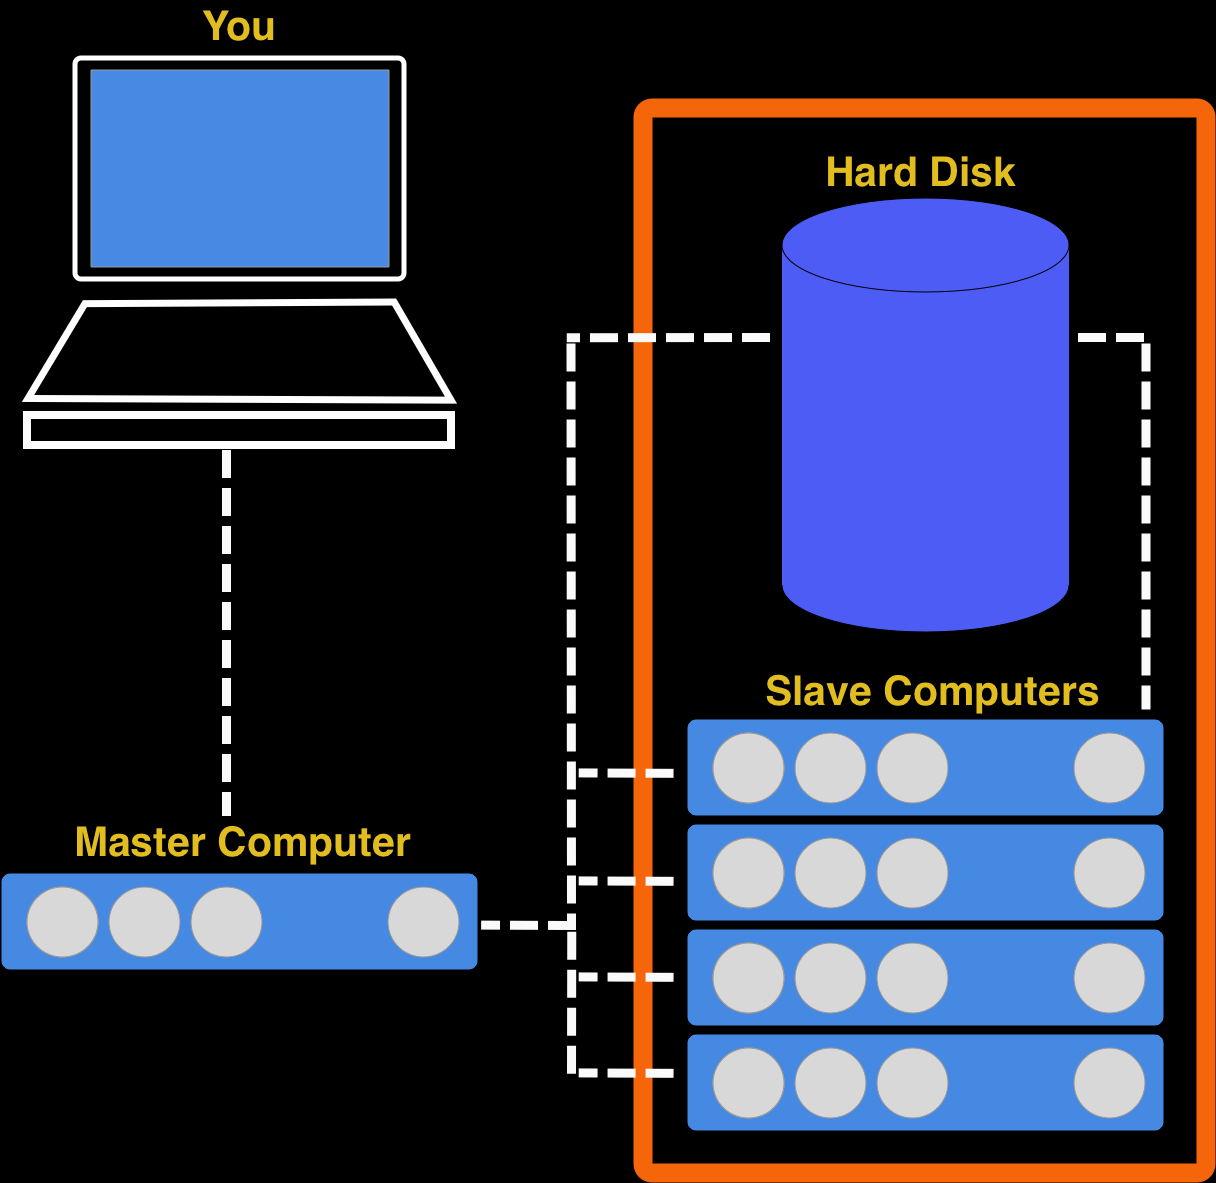
\includegraphics{hpc_graphic.png}

It shows the computer you are working at, the master computer and it's relation to the slave computers and the hard disk. Note that there is no way for you to contact the slaves directly, even though the slaves (or more properly `worker nodes') are where the actual job runs. So the workflow for running an HPC job goes like this

\begin{enumerate}
\def\labelenumi{\arabic{enumi}.}
\tightlist
\item
  Log into master (more usually called `submission node' )
\item
  Prepare a task for the submission node to send to the nodes
\item
  Submit the task to the submission node
\item
  Wait for the submission node to send the job to the worker nodes
\item
  Wait for the worker nodes to finish the job
\end{enumerate}

In the rest of this chapter we'll look at how to do these steps

\hypertarget{logging-into-the-submission-node}{%
\section{Logging into the submission node}\label{logging-into-the-submission-node}}

This is pretty straightforward, you need to use the \texttt{ssh} command to make a connection between your computer and the submission node. The TSL submission node has the address \texttt{hpc.tsl.ac.uk} so use this command

\begin{verbatim}
ssh hpc.tsl.ac.uk
\end{verbatim}

You'll be asked for a user name and password, it's your usual NBI details. When it's done you should see something like this

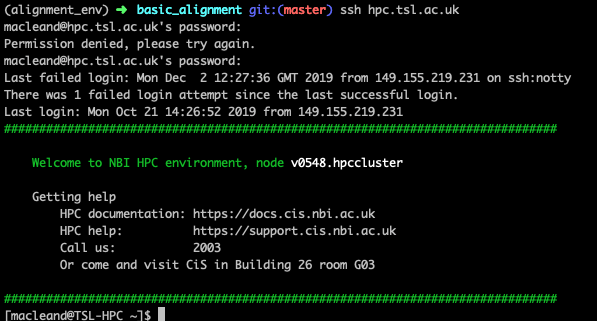
\includegraphics{login.png}

This terminal is now working on the submission node (you can tell from the prompt \texttt{macleand@TSL-HPC})

\hypertarget{preparing-a-job}{%
\section{Preparing a job}\label{preparing-a-job}}

To run a job we need to create a submission script. \texttt{nano} is available on the submission node, so we can use that. But what goes inside? Here's a typical one.

\begin{verbatim}
#!/bin/bash

#SBATCH -p tsl-short
#SBATCH --mem=16G
#SBATCH -c 4
#SBATCH -J alignments
#SBATCH --mail-type=begin,end,fail
#SBATCH --mail-user=dan.maclean@tsl.ac.uk
#SBATCH -o alignments.%j.out
#SBATCH -e slurm.%j.err

source minimap2-2.5
source samtools-1.9

srun minimap2 -ax sr ecoli_genome.fa ecoli_left_R1.fq ecoli_right_R2.fq | samtools view -S -h -b -q 25 -f 3 > aln.script.bam
\end{verbatim}

Not much of this is going to be familiar, but it isn't complicated.

The first line of this file \texttt{\#!/bin/bash} is one that should always be there. Always put it in and never worry about it again. It just tells the computer this file is a script.

\hypertarget{the-sbatch-options}{%
\subsection{\texorpdfstring{The \texttt{\#SBATCH} options}{The \#SBATCH options}}\label{the-sbatch-options}}

The second block of statements, all beginning \texttt{\#SBATCH} are the resource options for the job. It tells the submission node what resources the job needs to run. These need to go at the top of the script. Let's look at them individually.

\hypertarget{sbatch--p}{%
\subsubsection{\texorpdfstring{\texttt{\#SBATCH\ -p}}{\#SBATCH -p}}\label{sbatch--p}}

This tells the submission node which queue (or partition in the jargon) the job should run on. We have three basic partitions \texttt{tsl-short}, \texttt{tsl-medium} and \texttt{tsl-long}. The main difference is that jobs that run for a short time shouldn't be held back by jobs that run for ages, so the submission node uses this to run all of its jobs optimally.

\hypertarget{sbatch--c}{%
\subsubsection{\texorpdfstring{\texttt{\#SBATCH\ -c}}{\#SBATCH -c}}\label{sbatch--c}}

The number here tells the machine how many CPU's (processors) to use. Most tools will be able to make use of more than one and will run faster as a consequence. The job (usually) won't fail if you get this wrong, but it will take longer to start as it waits for more CPU's to come free.

\hypertarget{sbatch---mem}{%
\subsubsection{\texorpdfstring{\texttt{\#SBATCH\ -\/-mem=}}{\#SBATCH -\/-mem=}}\label{sbatch---mem}}

This tells the submission node how much memory your job will need to run. Jobs that exceed their stated memory by too much are killed. REquestiing the lowest possible memory means your job will be executed more quickly. Memory is requested in units of \texttt{G} gigabytes, usually.

\hypertarget{sbatch--j}{%
\subsubsection{\texorpdfstring{\texttt{\#SBATCH\ -J}}{\#SBATCH -J}}\label{sbatch--j}}

This is a helpful little name for you to identify your jobs with. eg \texttt{\#SBATCH\ -J\ my\_jobs}

\hypertarget{sbatch---mail-type}{%
\subsubsection{\texorpdfstring{\texttt{\#SBATCH\ -\/-mail-type=}}{\#SBATCH -\/-mail-type=}}\label{sbatch---mail-type}}

These are the times during the job that the submission node will email you to let you know of a status change in your job. Always use this option as presented for quickest information.

\hypertarget{sbatch---mail-user}{%
\subsubsection{\texorpdfstring{\texttt{\#SBATCH\ -\/-mail-user}}{\#SBATCH -\/-mail-user}}\label{sbatch---mail-user}}

This is simply the address your update emails will be sent to.

\hypertarget{sbatch--o-and-sbatch--e}{%
\subsubsection{\texorpdfstring{\texttt{\#SBATCH\ -o} and \texttt{\#SBATCH\ -e}}{\#SBATCH -o and \#SBATCH -e}}\label{sbatch--o-and-sbatch--e}}

These are the names of files that output and errors will be sent to. On a long running process the output can get long so it goes to a file, not the email. The weird \texttt{\%j} is a job ID number that uniquely identifies the job.

\hypertarget{the-source-options}{%
\subsection{\texorpdfstring{The \texttt{source} options}{The source options}}\label{the-source-options}}

The next lines all begin with the word \texttt{source} followed by some software name. No software is loaded into the worker nodes by default, so we need to say which tools we want to use. Do this by using the \texttt{source} keyword followed by the software name, e.g \texttt{source\ BLAST-2.2.2}. Many versions of the same tool are available on the HPC, and are differentiated by the version number at the end. You can see which software is available to source by typing \texttt{source} then hitting the tab key twice. It should give a very long list of tools.

\hypertarget{the-srun-command}{%
\subsection{\texorpdfstring{The \texttt{srun} command}{The srun command}}\label{the-srun-command}}

Finally, we get to the actual commands we want to run. This is exactly as we did before but with the command \texttt{srun} in front.

\hypertarget{submitting-with-sbatch}{%
\section{\texorpdfstring{Submitting with \texttt{sbatch}}{Submitting with sbatch}}\label{submitting-with-sbatch}}

All of this information should be saved in a single script. You can call it what you want, but use the extension \texttt{.sh}. Once you've got this script, you can ask the submission node to add your job to the queue with \texttt{sbatch}. This doesn't go in the script, it goes on the command-line, so if you'd added all the details above to a file called \texttt{do\_my\_alignments.sh} you can submit it by typing \texttt{sbatch\ do\_my\_alignments.sh}

\hypertarget{checkout-tasks}{%
\section{Checkout tasks}\label{checkout-tasks}}

So that's all you need to know to submit a job. Let's test how that works by creating a simple job and running that. Then we'll try a bigger alignment job. These are

\begin{enumerate}
\def\labelenumi{\arabic{enumi}.}
\tightlist
\item
  Create a job using a submission script that runs this command \texttt{date}. Check what the \texttt{date} command does on the command line. Note that it runs very quickly (is a short job) and uses very little memory (\textless{} 1G) and only needs one CPU.
\item
  What happened to the output? Check the contents of your directory when the job is done and examine the new files (\texttt{less} is useful for this).
\item
  Explicitly create an output file by running this command through the HPC instead \texttt{date\ \textgreater{}\ date.txt}. What is the contents of the folder now? What effect did explicitly naming an output file have. What is the \texttt{slurm\_xxxx.out} file for?
\item
  Run an alignment job using the information we learned in the earlier chapters. The reference file \texttt{ecoli\_genome.fa}, \texttt{ecoli\_left\_R1.fq}, \texttt{ecoli\_right\_R2.fq} are available in the HPC filesystem in the folder. \texttt{/tsl/data/reads/bioinformatics/tutorial/alignments/}
\end{enumerate}

\hypertarget{further-reading-4}{%
\section{Further Reading}\label{further-reading-4}}

You can see more information about the cluster submission system and options at the CiS \href{https://docs.cis.nbi.ac.uk/display/CIS/Run+a+simple+job+on+the+cluster}{documentation site}

\bibliography{book.bib,packages.bib}


\end{document}
